\section{Malware Temporal Properties}
\label{sec:temporal}

This section presents our study of the temporal properties of VirusTotal malwares
and answers three fundamental questions: 
how many malware families appear everyday, 
{\color{red} (Work 2)
what lifetime of malwares on VirusTotal distributes,  
}
and whether or not malwares occur in bursts.
To answer the last question, we design a new caching mechanism 
that can be used for both offline and online malware predictions.
This cache-based malware prediction technique can predict which malware families will appear in the near future with high precision.

\begin{figure*}[!htb]
\minipage{0.31\textwidth}
  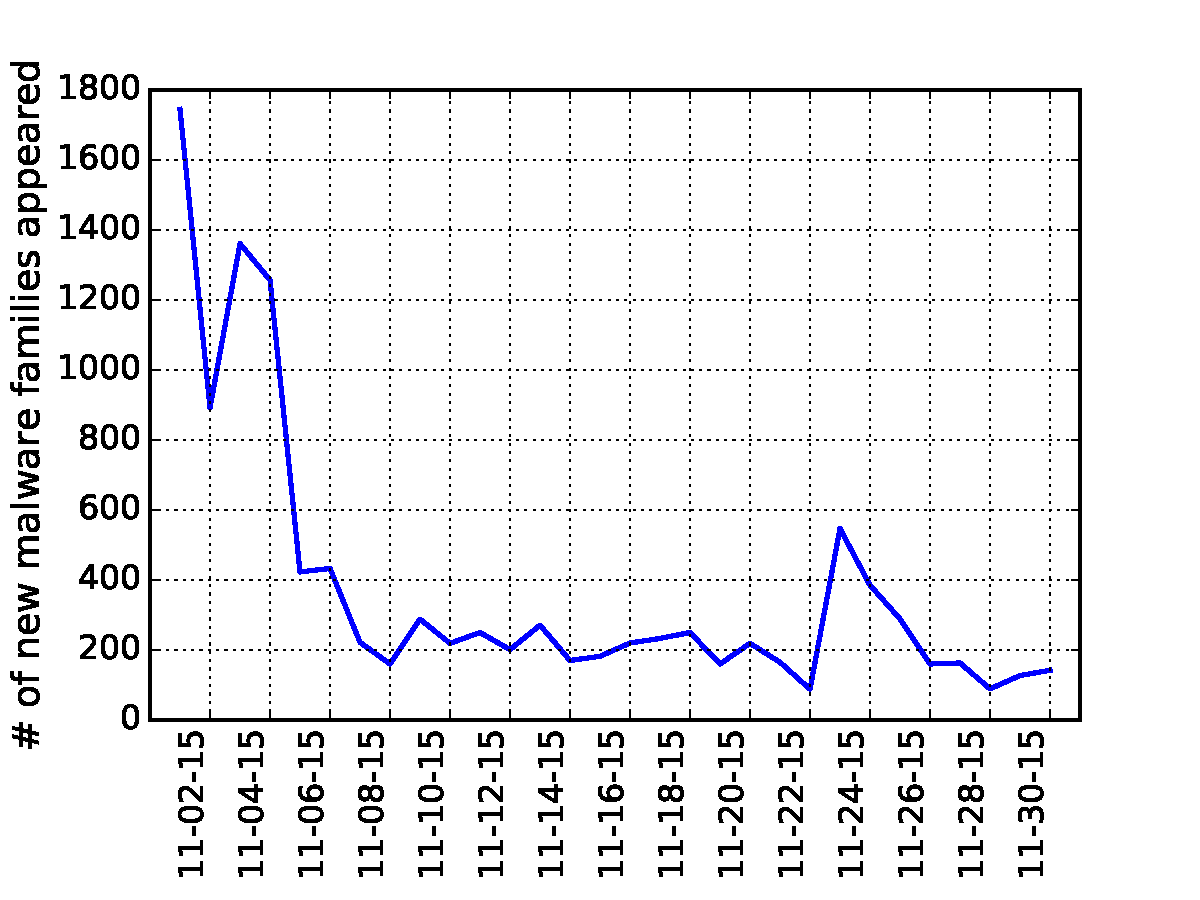
\includegraphics[width=\linewidth]{figure/new_family}
\mycaption{fig:new}{New malware families on VirusTotal in November 2015.}
{
The number of new malware families we observed every day in November 2015.
}
  %\label{fig:overlap}
\endminipage\hfill
\minipage{0.31\textwidth}
  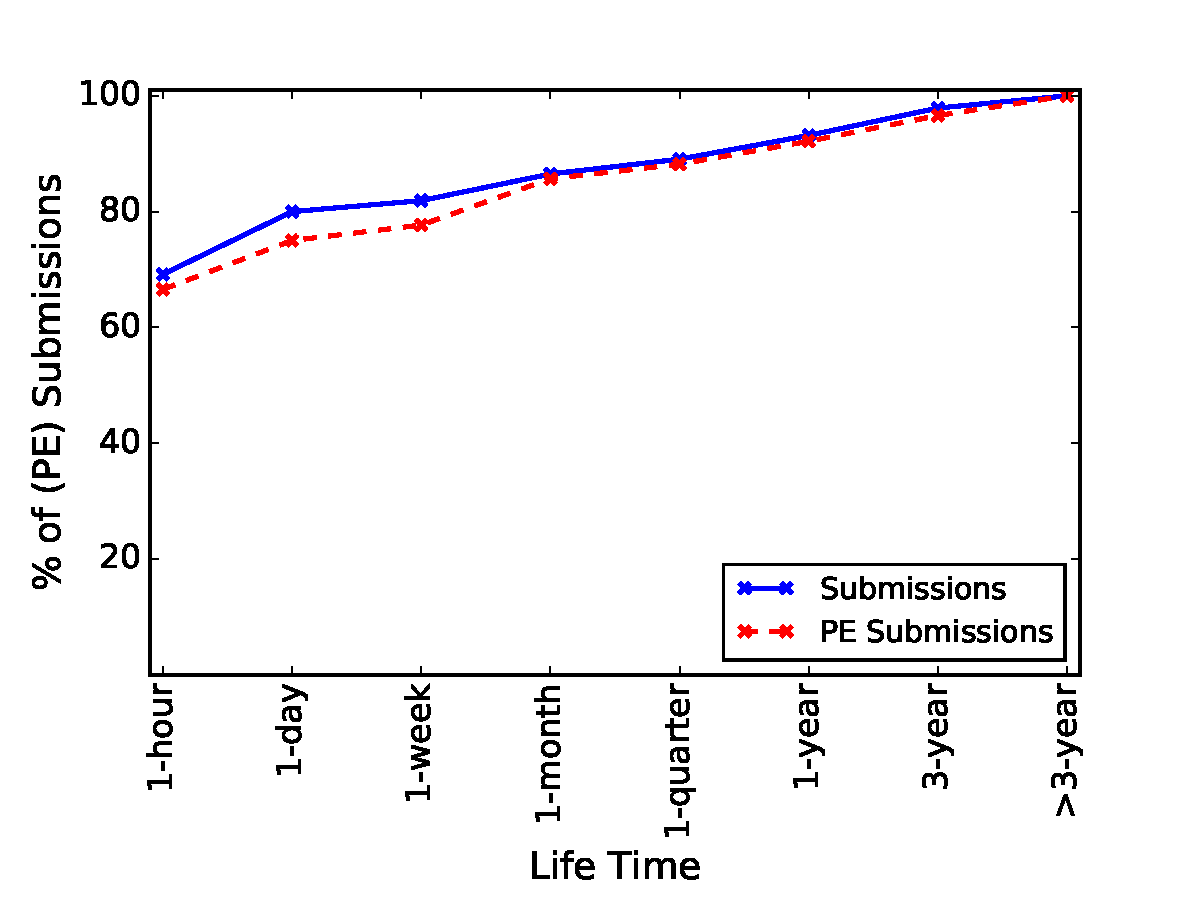
\includegraphics[width=\linewidth]{figure/lifetime}
 \mycaption{fig:life}{Malwares' lifetime in November 2015.}
{
Cumulative distribution of lifetime for malwares with more than one submission in November 2015.
}
  %\label{fig:maxUncover}
\endminipage\hfill
\minipage{0.31\textwidth}%
  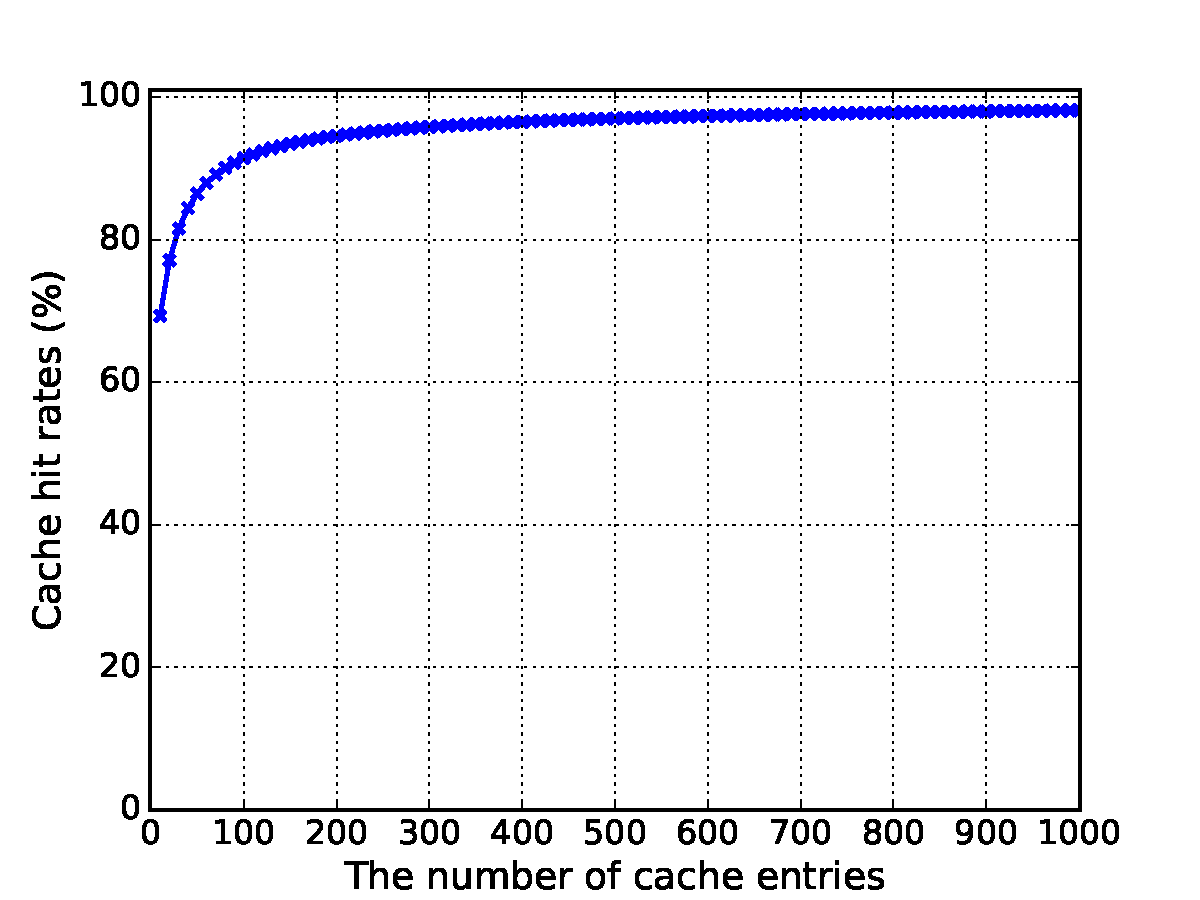
\includegraphics[width=\linewidth]{figure/LRU}
  \mycaption{fig:cache}{Relation between cache hit rate and cache size.}
{Cache hit rate under different values of cache size from 10 to 1000.}
  %\label{fig:aveUncover}
\endminipage\hfill

\vspace{-0.1in}
\end{figure*}

\begin{figure*}[!htb]
\minipage{0.31\textwidth}
  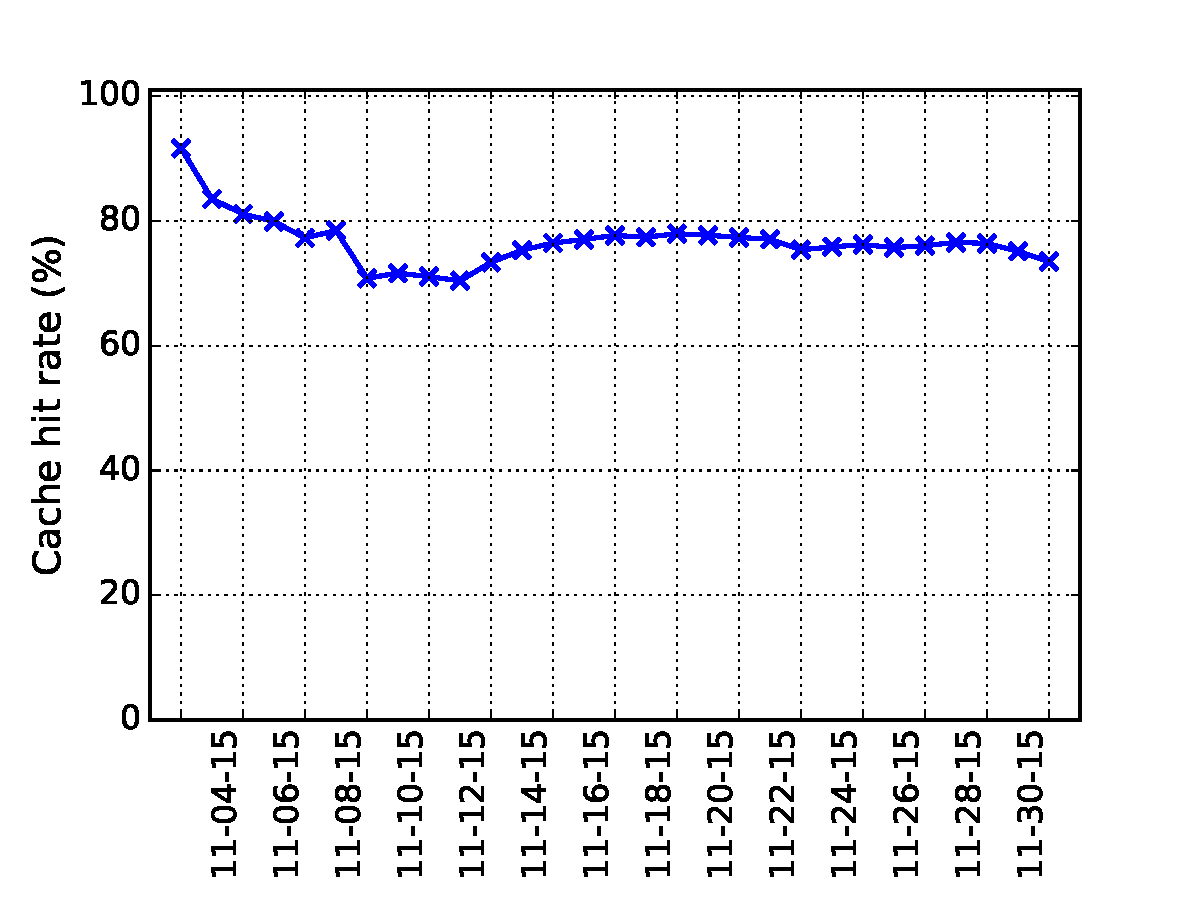
\includegraphics[width=\linewidth]{figure/LRU_day}
\mycaption{fig:batchcache}{Cache hit rate in November 2015.}
{
Cache hit rate every day in November 2015 if we only update cache content at the end of every day.
}
  %\label{fig:overlap}
\endminipage\hfill
\minipage{0.31\textwidth}
  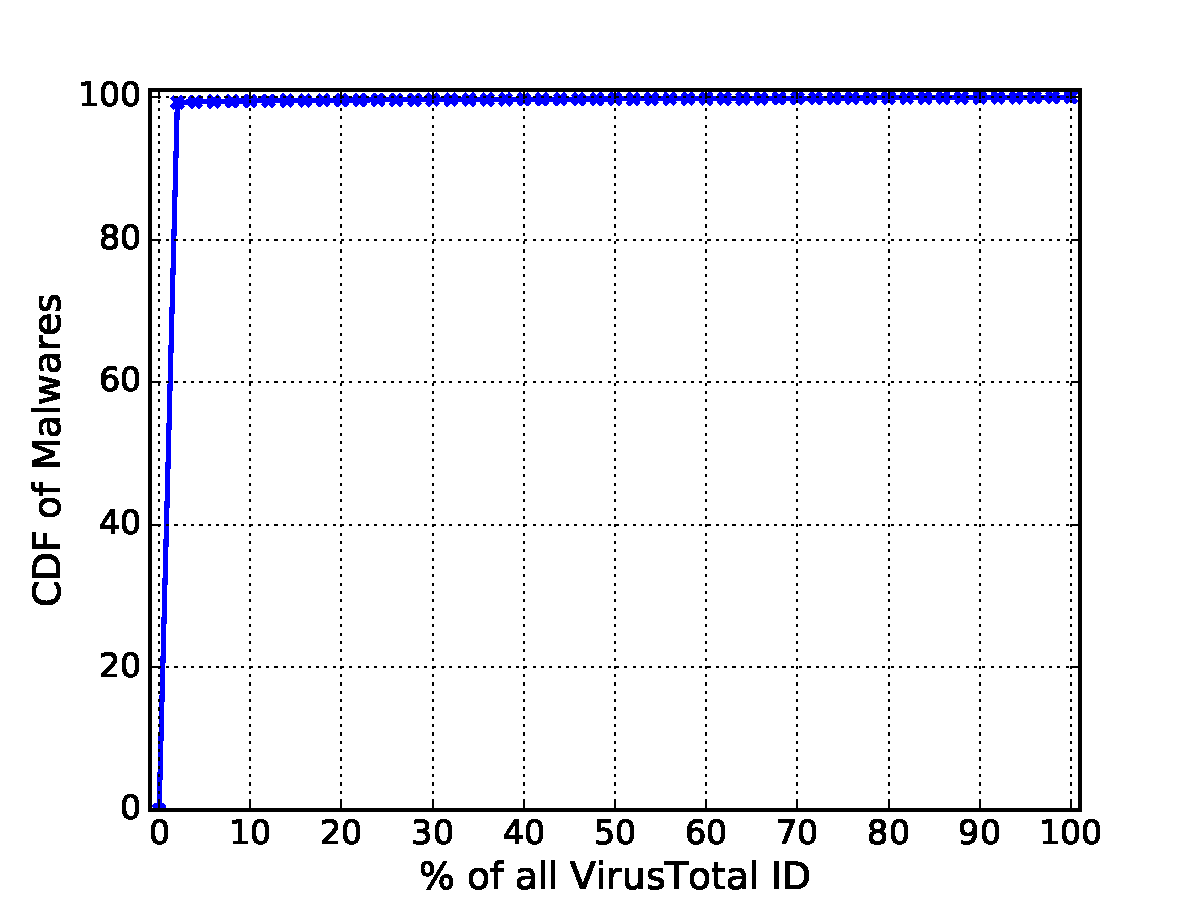
\includegraphics[width=\linewidth]{figure/id}
 \mycaption{fig:id}{Skewness of malware submissions from different users in November 2015.}
{Cumulative distribution of malwares submitted by different users in November 2015.}
  %\label{fig:maxUncover}
\endminipage\hfill
\minipage{0.31\textwidth}%
  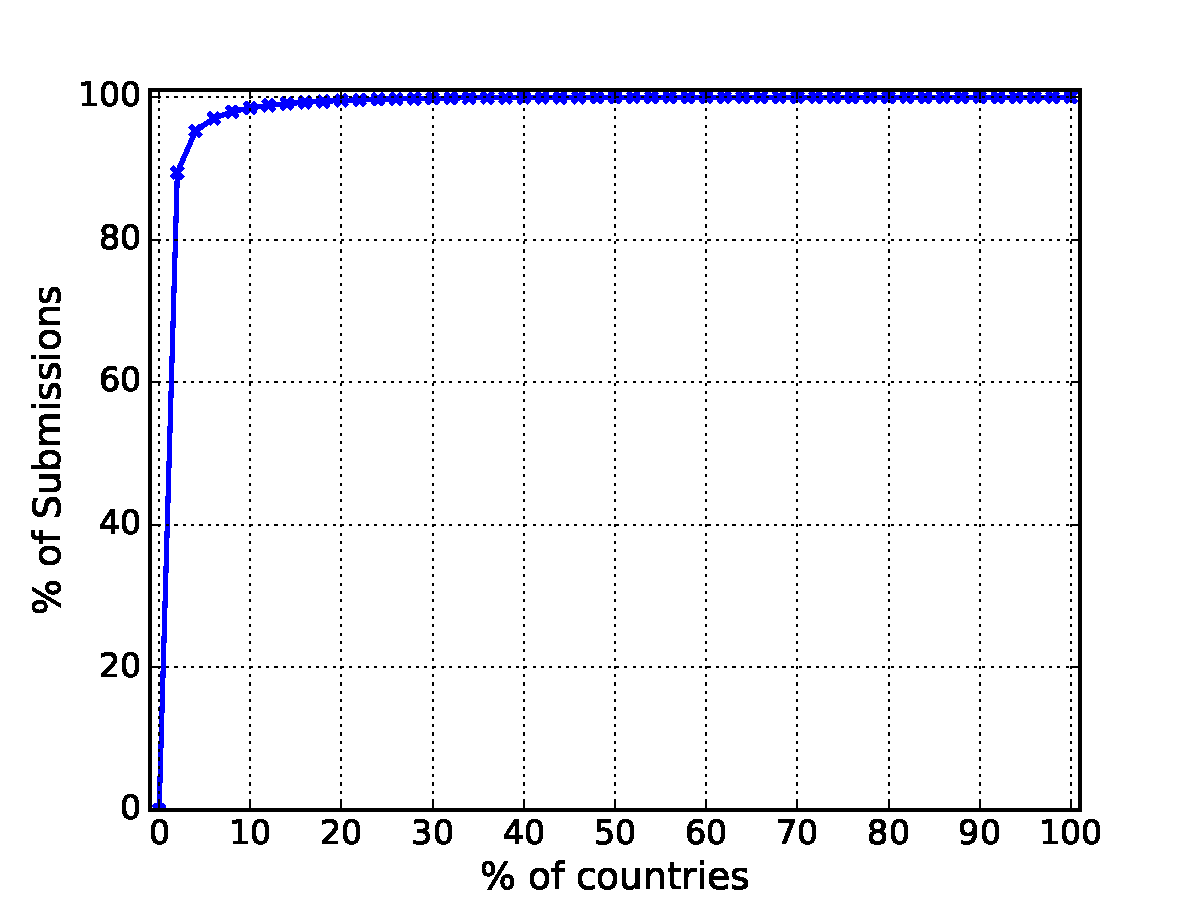
\includegraphics[width=\linewidth]{figure/country}
  \mycaption{fig:country}{Skewness of malware submissions from different countries in November 2015.}
{Cumulative distribution of malwares submitted from different countries in November 2015.}
  %\label{fig:aveUncover}
\endminipage\hfill

\vspace{-0.1in}
\end{figure*}

We first study how many new malware families appear everyday. 
Figure~\ref{fig:new} shows the number of new malware families appearing on each day in November 2015. 
Since we do not include data before November 1, 
there are more new malware families in the first few days.
After that, the number of new malware families becomes stable, 
falling into a range between 100 and 400. 
In total, there are 11302 malware families in this time period. 

{\bf Observation 1:} 
{\em 100-400 new malware families appear each day.}

%\begin{figure}[t!]
\begin{center}
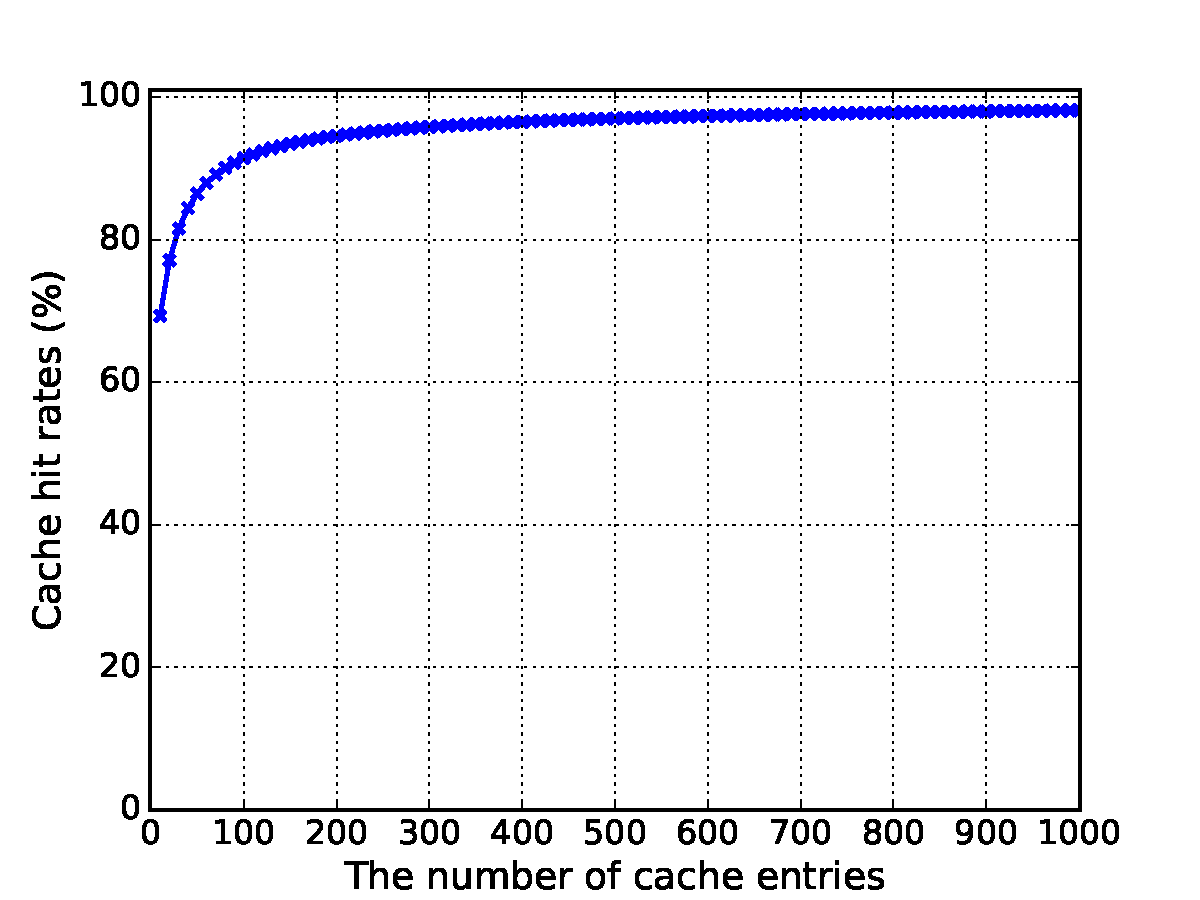
\includegraphics[width=2.5in]{figure/LRU}
\mycaption{fig:cache}{Relation between cache hit rate and cache size.}
{How cache hit rate changes with the change of cache size from 10 to 1000.}
%\label{fig:cache}
\end{center}
\end{figure}
%\begin{figure}[t!]
\begin{center}
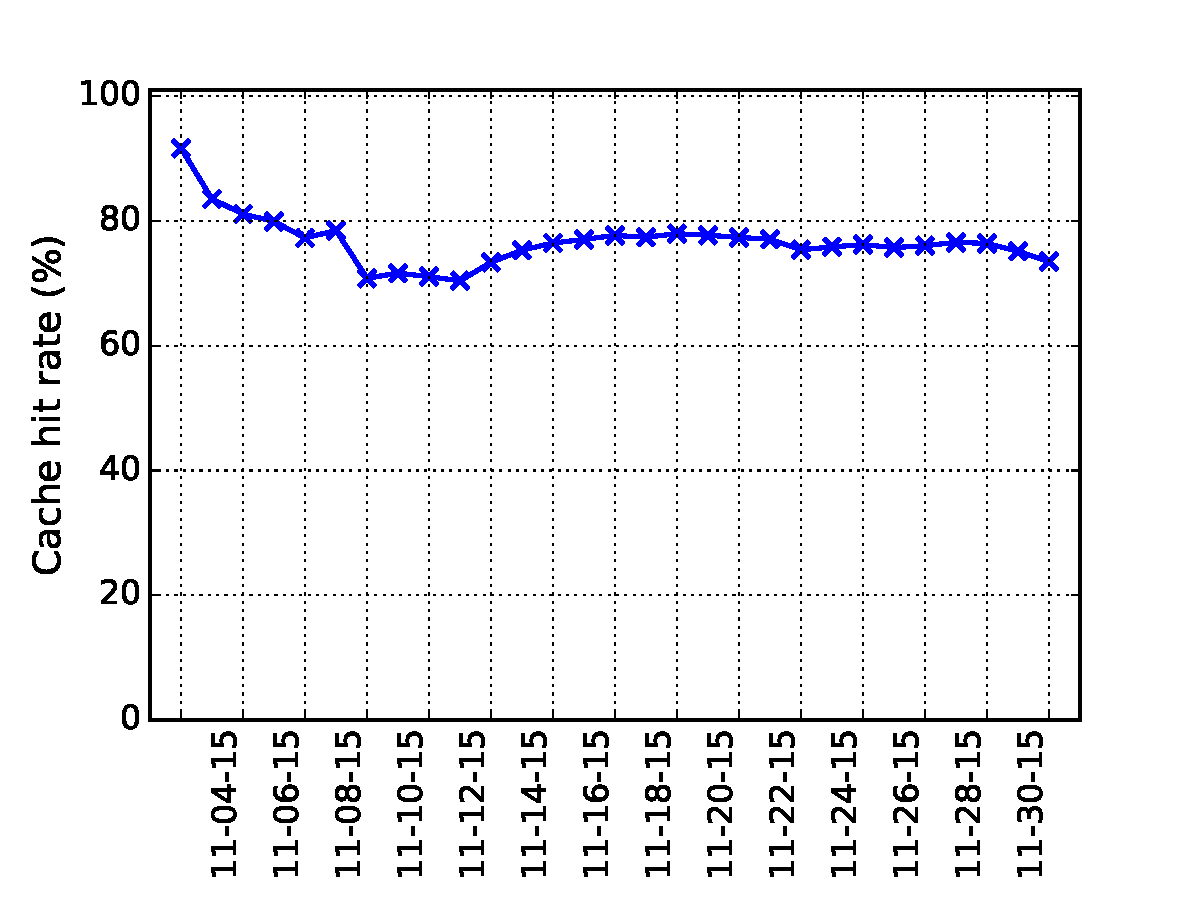
\includegraphics[width=2.5in]{figure/LRU_day}
\mycaption{fig:batchcache}{Cache hit rate in November 2015.}
{Cache hit rate every day in November 2015 if we only update cache content at the end of every day.}
%\label{fig:batchcache}
\end{center}
\vspace{-0.1in}
\end{figure}



{\color{red} (Work 2)
An interesting property worth studying is how long a malware lives. 
Finding the exact answer to this question is extremely difficult, since there 
is no log of when a malware comes into existence and when it extincts.
Here, we use the VirusTotal data to have a peek into this question.
Specifically, we use the tiem span from when the first submission of a malware to VirusTotal happens
to the time of its last submission
to provide a rough estimation of the life time of this malwares.
Figure~\ref{fig:life} plots the cummulative distribution of the calculated submission time span of malwares with more than one submission.
89.68\% malwares are only submitted once.
Other than these malwares, 0.004\% malwares have submission span within an hour, 
0.17\% span from one hour to one day, and 8.39\% span more than one week.


{\bf Observation 2:}
{\em A fair amount of malwares live longer than one week.} % need to conclude this based on the above numbers

}


Finally, we investigate whether malwares behave temporal locality.
Temporal locality is an important metric that can guide the 
prediction of near-future malwares.

Specifically, we analyze how bursty malwares in the same family appear.  
Inspired by previous usage of cache mechanisms in predicting bugs~\cite{predicting},
we design a new cache mechanism to study the burstiness of malwares.

This caching mechanism can be used to analyze historical malware reports offline 
as well as to analyze online malwares and predict near-future malware occurrences.

We view malware submission reports as a stream of inputs 
and feed the stream into a cache. 
Each input (\ie, each report) is associated with an address (the family it belongs to) and a time (the submission time of the file).
Thus, a cache hit means that the new report belongs to a family that is currently in the cache,
\ie, the new input has the same address as an entry in the cache.
Therefore, a high cache hit rate implies that the occurrence of malwares exhibit temporal locality.

As with general cache mechanisms such as CPU caches and file system buffer caches, 
there are several parameters to tune in a cache.
The cache block size, or cache line size, controls the granularity of cache management, 
\ie, how many entries are inserted into and evicted from cache together.
Cache prefetching loads spatially close entries into caches in advance. 
Cache replacement policy controls what entries to evict when cache is full.
{\color{red} (Writing 9)
We use a simple cache setting in our evaluation. 
We fix the cache block size to be one, no prefetching, 
and use the LRU replacement policy.
We leave the exploration of the effect of other cache configurations for future work. 

Our malware family cache works as follows.
We start with an empty cache. 
For a new file submission, if the malware family is already in the cache, 
we move the hit cache entry to the front of our cache entry list. 
If the new malware family is not in the cache, 
we create a new cache entry and add it to the front of the cache entry list.
If the cache is full, we evict the entry at the end of the list. 
%The cache hit rate is calculated as follows: 
}

%$$ \mbox{hit rate} = \dfrac{\mbox{\# of hits}}{\mbox{\# of hits + \# of misses}}$$

We implemented this malware family cache using Python
and conducted experiments on an AWS c4.4xlarge virtual machine, 
which contains 16 virtual CPUs and 30\,GB memory.

We conducted two experiments. 
The first experiment explores how the cache hit rate changes with the number of cache entries. 
We change the cache size from 10 to 1000. 
As shown in Figure~\ref{fig:cache}, the hit rate grows from 69.31\% to 98.14\%. 
When using more than 80 cache entries, which is less than 1\% of the total number of malware families, the cache hit rate rises above 90\%, 
and when using more than 230 cache entries, which is less than 3\% of the total number of malware families, 
the cache hit rate rises above 95\%. 
{\color{red} (Writing 8)
The high cache hit rate and the small cache size confirm that malwares occur in bursts.
}

{\bf Observation 3:} 
{\em The occurrence of malwares in each family has strong temporal locality.}  

{\color{red} (Writing 7)
In offline prediction, malwares encountered in each client site are merged together. 
These data are used to predict which malware family would appear in the near future in a large scale.
Malwares encountered in one client site can be viewed as a random sample of all malwares. 
If we can predict malware occurrence online, we could apply personalized defense mechanism and malware detection mechanism on the client side. 
}
To support online malware occurrence prediction, it is essential to lower the 
performance overhead of running our cache mechanism.
To this end, we lower the cache content update frequency from once per malware report to once per day.
That is, we keep cache content unchanged to count cache hits and cache misses each day and update the cache content at the end of each day.
In this second experiment, we fix the cache size to 200. 
{\color{red} (Writing 1)
Figure~\ref{fig:batchcache} shows prediction rate by using next day’s data. 
Most cache hit rate is above 70\%,
showing that even when lowering performance overhead, \ie, updating cache content once a day, 
our cache mechanism still achieves a good estimation of malware occurrences.
}   
{\color{red} (Writing 9)
We do not need to combine malwares encountered in each client site and send out updated cache content frequently. Cache-based malware prediction can be used in an online scenario. 
}

{\color{red} (Work 6)
We also study which malware families cause more cache misses 
and have bad prediction results. 
We count cache misses for each malware family, 
and consider a family with more than half malwares causing cache misses as family with bad prediction results. 
We find that whether a family has bad prediction results is related to the number of malwares it contains. 
When cache size is 100, the largest number of malwares contained in one family with bad prediction results is 2307. 
When cache size is 1000, the largest number of malwares contained in one family with bad prediction results is 126. 
}


